\newpage

\section{Additional experiments for section~\ref{sec:verifying_calibration}}
\label{sec:verifying_calibration_appendix_experiments}

In Section~\ref{sec:verifying_calibration} we ran an experiment on CIFAR-10 to show that the debiased estimator gives estimates closer to the true calubration error than the plugin estimator. To give more insight into this, Figure~\ref{fig:histograms_estimators_bins} shows a histogram of the absolute difference between the estimates and ground truth for the plugin and debiased estimator, over the 1,000 resamples, when we use $B = 10$ or $B = 100$ bins. For $B = 10$ bins it is not completely clear which estimator is doing better but the debiased estimator avoids very bad estimates. However, when $B = 100$, the debiased estimator produces estimates much closer to the ground truth ($0$ on the x-axis).

We also ran a multiclass calibration experiment on CIFAR-10 to show that our estimator allows us to select models with a lower mean-squared error subject to a given calibration constraint. In this case we split the validation set into $\calset{}$ and $\verifset{}$ of size 6000 and 4000 respectively, and recalibrated a trained model on $\calset{}$. On $\verifset{}$, we estimate the calibration error using the plugin and debiased estimators and use 100 Bootstrap resamples to compute a 90\% upper confidence bound on the estimate (from the variance of the Bootstrap samples). We compute the mean-squared error and the upper bounds on the calibration error for $B = 10, 15, \dots, 100$ and show the Pareto curve in Figure~\ref{fig:mse_vs_ce_estimator}. Figure~\ref{fig:mse_vs_ce_estimator} shows that for any desired calibration error, the debiased estimator enables us to pick out models with a better mean-squared error. For example, if we want a model with $\ell_2$ calibration error less than $1.5\%$, the debiased estimator tells us we can confidently use 100 bins, while relying on the plugin estimator only lets us use 15 bins and incurs a 13\% higher mean-squared error.

% Note that in our theoretical results in Section~\ref{sec:verifying_calibration}, we focused on hypothesis testing, using the estimator to test whether a model has calibration error $\leq \epsilon$ or not. However, the 

% \pl{say explicitly that we never say 'not calibrated'; there's a disconnect between the theory, which requires $r$ and $\epsilon$ and what we're doing here}

\begin{figure}
  \centering
  \centering
     \begin{subfigure}[b]{0.45\textwidth}
         \centering
         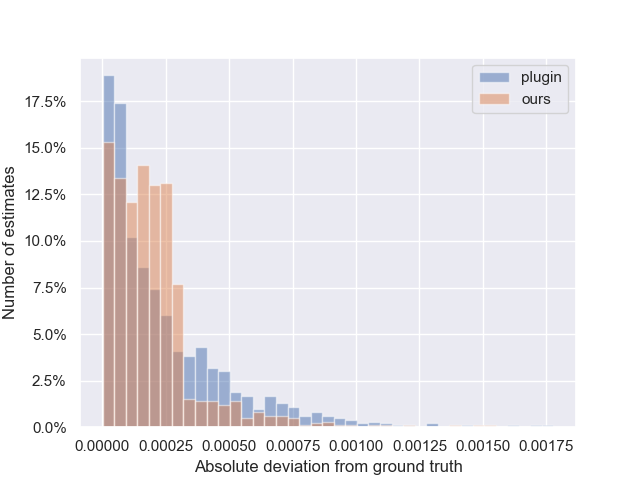
\includegraphics[width=\textwidth]{histogram_estimators_10_bins.png}
         \caption{$B$ = 10 bins}
     \end{subfigure}
     \hfill
     \begin{subfigure}[b]{0.45\textwidth}
         \centering
         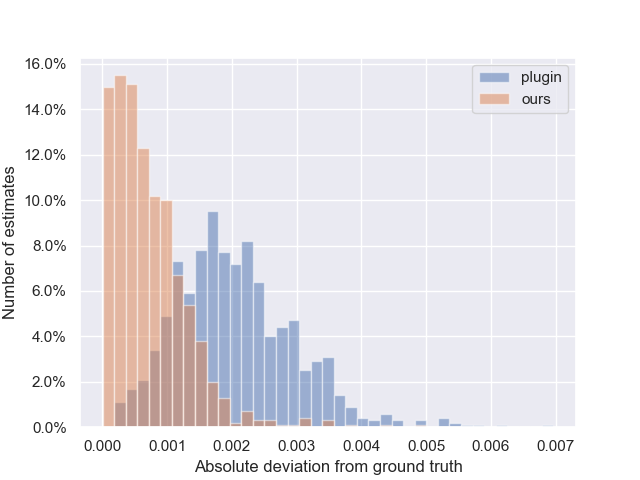
\includegraphics[width=\textwidth]{histogram_estimates_100_bins.png}
         \caption{$B = 100$ bins}
     \end{subfigure}
  \caption{Histograms of the absolute value of the difference between estimated and ground truth $\lsquared$ calibration errors ($0$ on the x-axis). For $B = 10$ bins, the results are mixed but we avoid very bad estimates. For $B=100$ our estimates are much closer to ground truth.}
  \label{fig:histograms_estimators_bins}
\end{figure}

\begin{figure}
  \centering
  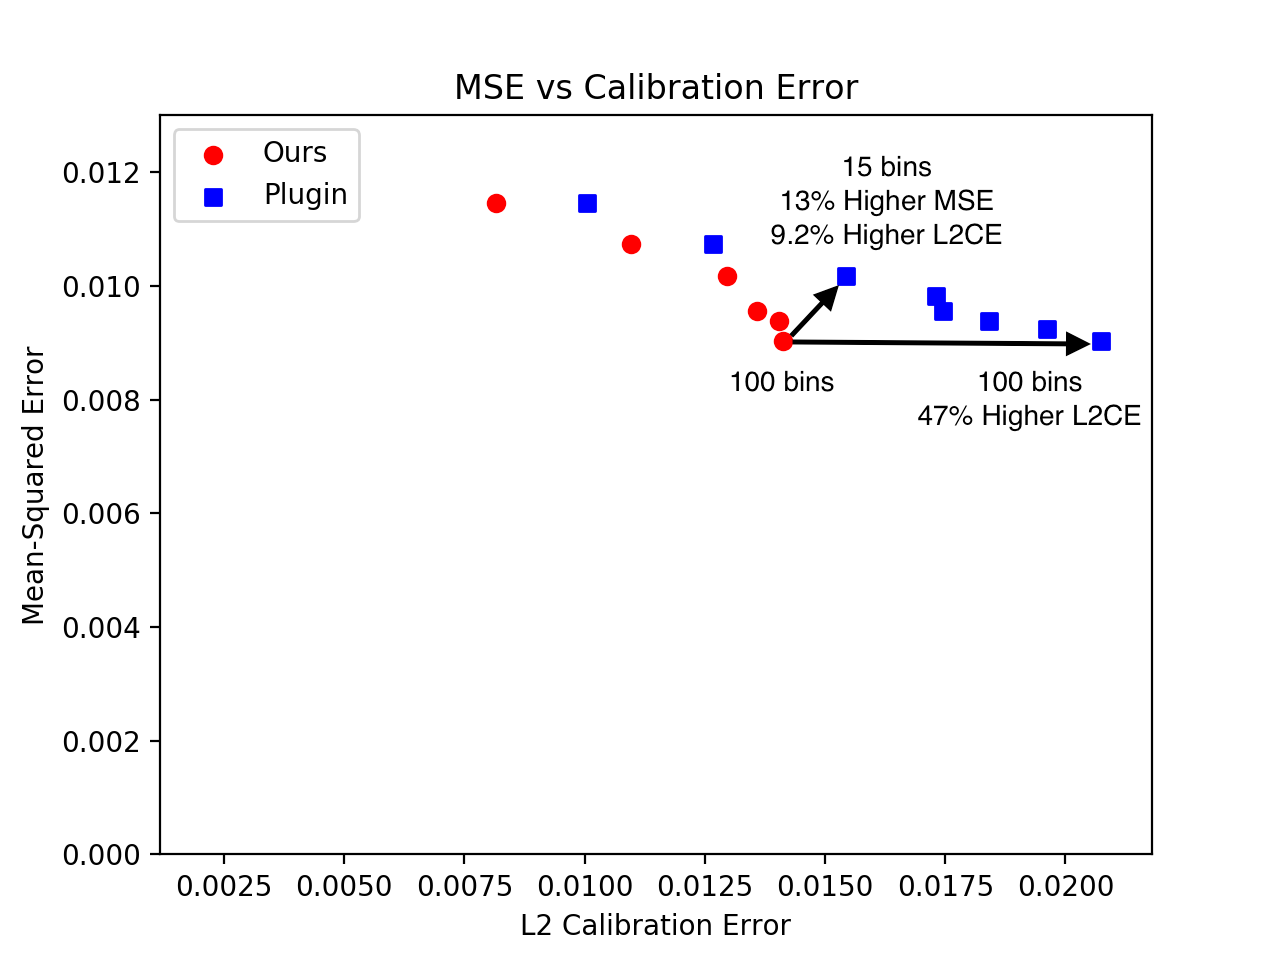
\includegraphics[width=0.9\textwidth]{mse_vs_verified_error_plugin_vs_ours.png}
  \caption{Plot of mean-squared error against 90\% upper bounds on the calibration error computed by the debiased estimator and the plugin estimator, when we vary the number of bins $B$. For a given calibration error, our estimator enables us to choose models with a better mean-squared error. If we want a model with $\ell_2$ calibration error less than 0.015, the debiased estimator tells us we can confidently use 100 bins, while relying on the plugin estimator only lets us use 15 bins and incurs a 13\% higher mean-squared error.}
  \label{fig:mse_vs_ce_estimator}
\end{figure}

